\chapter{Software}

\color{blue}
\section{ROS}
The Robot Operating System, henceforth called ROS, is middleware created with the goal of making the communication infrastructure of robot technology easier.\\
At the lowest level, ROS provides the infrastructure of inter-process messages. The code is written into nodes, that represent each process. Every node can then subscribe or publish to other nodes in the network and can then freely communicate doing operations. In between each talking node there is either a service, often used for 1-node/1-node communication, or topics which are used for communication between multiple nodes to multiple subscribers. The nodes \textit{send and receive} messages, which are the blocks of code containing the \textit{sent and received} information. \\
The ROS Master handle: registration, naming and tracks and enable individual ROS nodes to locate one another.

\begin{figure}[H]
    \centering
    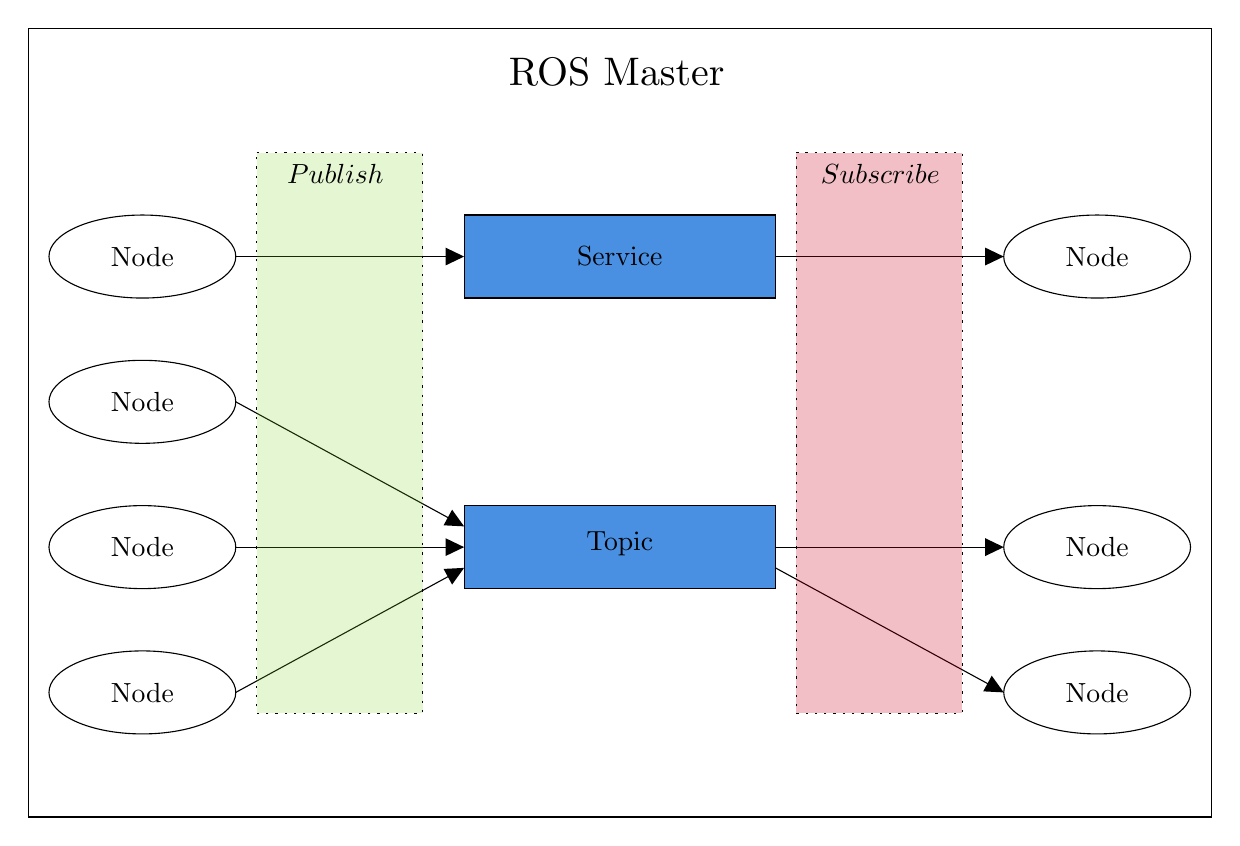
\begin{tikzpicture}[x=0.75pt,y=0.75pt,yscale=-1,xscale=1]
    %uncomment if require: \path (0,426); %set diagram left start at 0, and has height of 426
    
    %Shape: Ellipse [id:dp45078602668243484] 
    \draw   (10,140) .. controls (10,128.95) and (30.15,120) .. (55,120) .. controls (79.85,120) and (100,128.95) .. (100,140) .. controls (100,151.05) and (79.85,160) .. (55,160) .. controls (30.15,160) and (10,151.05) .. (10,140) -- cycle ;
    
    %Shape: Ellipse [id:dp9549841346304726] 
    \draw   (10,210) .. controls (10,198.95) and (30.15,190) .. (55,190) .. controls (79.85,190) and (100,198.95) .. (100,210) .. controls (100,221.05) and (79.85,230) .. (55,230) .. controls (30.15,230) and (10,221.05) .. (10,210) -- cycle ;
    
    %Shape: Ellipse [id:dp9558643533491318] 
    \draw   (10,280) .. controls (10,268.95) and (30.15,260) .. (55,260) .. controls (79.85,260) and (100,268.95) .. (100,280) .. controls (100,291.05) and (79.85,300) .. (55,300) .. controls (30.15,300) and (10,291.05) .. (10,280) -- cycle ;
    
    %Shape: Ellipse [id:dp6803958977785123] 
    \draw   (10,350) .. controls (10,338.95) and (30.15,330) .. (55,330) .. controls (79.85,330) and (100,338.95) .. (100,350) .. controls (100,361.05) and (79.85,370) .. (55,370) .. controls (30.15,370) and (10,361.05) .. (10,350) -- cycle ;
    
    %Shape: Ellipse [id:dp6544758566888991] 
    \draw   (470,140) .. controls (470,128.95) and (490.15,120) .. (515,120) .. controls (539.85,120) and (560,128.95) .. (560,140) .. controls (560,151.05) and (539.85,160) .. (515,160) .. controls (490.15,160) and (470,151.05) .. (470,140) -- cycle ;
    
    %Shape: Ellipse [id:dp7539921241856691] 
    \draw   (470,280) .. controls (470,268.95) and (490.15,260) .. (515,260) .. controls (539.85,260) and (560,268.95) .. (560,280) .. controls (560,291.05) and (539.85,300) .. (515,300) .. controls (490.15,300) and (470,291.05) .. (470,280) -- cycle ;
    
    %Shape: Ellipse [id:dp9196266586607387] 
    \draw   (470,350) .. controls (470,338.95) and (490.15,330) .. (515,330) .. controls (539.85,330) and (560,338.95) .. (560,350) .. controls (560,361.05) and (539.85,370) .. (515,370) .. controls (490.15,370) and (470,361.05) .. (470,350) -- cycle ;
    
    %Shape: Rectangle [id:dp7344023572727392] 
    \draw  [fill={rgb, 255:red, 74; green, 144; blue, 226 }  ,fill opacity=1 ] (210,120) -- (360,120) -- (360,160) -- (210,160) -- cycle ;
    %Shape: Rectangle [id:dp6597158053967722] 
    \draw  [fill={rgb, 255:red, 74; green, 144; blue, 226 }  ,fill opacity=1 ] (210,260) -- (360,260) -- (360,300) -- (210,300) -- cycle ;
    %Straight Lines [id:da6863831588778817] 
    \draw    (100,210) -- (208.24,269.04) ;
    \draw [shift={(210,270)}, rotate = 208.61] [fill={rgb, 255:red, 0; green, 0; blue, 0 }  ][line width=0.75]  [draw opacity=0] (8.93,-4.29) -- (0,0) -- (8.93,4.29) -- cycle    ;
    
    %Straight Lines [id:da12403607448981524] 
    \draw    (100,280) -- (208,280) ;
    \draw [shift={(210,280)}, rotate = 180] [fill={rgb, 255:red, 0; green, 0; blue, 0 }  ][line width=0.75]  [draw opacity=0] (8.93,-4.29) -- (0,0) -- (8.93,4.29) -- cycle    ;
    
    %Straight Lines [id:da03781151995197041] 
    \draw    (100,350) -- (208.24,290.96) ;
    \draw [shift={(210,290)}, rotate = 511.39] [fill={rgb, 255:red, 0; green, 0; blue, 0 }  ][line width=0.75]  [draw opacity=0] (8.93,-4.29) -- (0,0) -- (8.93,4.29) -- cycle    ;
    
    %Straight Lines [id:da1441202280359899] 
    \draw    (360,280) -- (468,280) ;
    \draw [shift={(470,280)}, rotate = 180] [fill={rgb, 255:red, 0; green, 0; blue, 0 }  ][line width=0.75]  [draw opacity=0] (8.93,-4.29) -- (0,0) -- (8.93,4.29) -- cycle    ;
    
    %Straight Lines [id:da48075246645909897] 
    \draw    (360,290) -- (468.24,349.04) ;
    \draw [shift={(470,350)}, rotate = 208.61] [fill={rgb, 255:red, 0; green, 0; blue, 0 }  ][line width=0.75]  [draw opacity=0] (8.93,-4.29) -- (0,0) -- (8.93,4.29) -- cycle    ;
    
    %Straight Lines [id:da029111479488499903] 
    \draw    (100,140) -- (208,140) ;
    \draw [shift={(210,140)}, rotate = 180] [fill={rgb, 255:red, 0; green, 0; blue, 0 }  ][line width=0.75]  [draw opacity=0] (8.93,-4.29) -- (0,0) -- (8.93,4.29) -- cycle    ;
    
    %Straight Lines [id:da3328719481411202] 
    \draw    (360,140) -- (468,140) ;
    \draw [shift={(470,140)}, rotate = 180] [fill={rgb, 255:red, 0; green, 0; blue, 0 }  ][line width=0.75]  [draw opacity=0] (8.93,-4.29) -- (0,0) -- (8.93,4.29) -- cycle    ;
    
    %Shape: Rectangle [id:dp8244335454881859] 
    \draw  [fill={rgb, 255:red, 208; green, 2; blue, 27 }  ,fill opacity=0.25 ][dash pattern={on 0.84pt off 2.51pt}] (370,90) -- (450,90) -- (450,360) -- (370,360) -- cycle ;
    %Shape: Rectangle [id:dp5835701508493467] 
    \draw  [fill={rgb, 255:red, 126; green, 211; blue, 33 }  ,fill opacity=0.2 ][dash pattern={on 0.84pt off 2.51pt}] (110,90) -- (190,90) -- (190,360) -- (110,360) -- cycle ;
    %Shape: Rectangle [id:dp734740621343706] 
    \draw   (0,30) -- (570,30) -- (570,410) -- (0,410) -- cycle ;
    
    % Text Node
    \draw (55,140) node  [align=left] {Node};
    % Text Node
    \draw (55,210) node  [align=left] {Node};
    % Text Node
    \draw (55,280) node  [align=left] {Node};
    % Text Node
    \draw (55,350) node  [align=left] {Node};
    % Text Node
    \draw (515,140) node  [align=left] {Node};
    % Text Node
    \draw (515,350) node  [align=left] {Node};
    % Text Node
    \draw (515,280) node  [align=left] {Node};
    % Text Node
    \draw (285,278.5) node  [align=left] {Topic};
    % Text Node
    \draw (285,140) node  [align=left] {Service};
    % Text Node
    \draw (148,100) node   {$Publish$};
    % Text Node
    \draw (415,100) node   {$Subscribe\ \ $};
    % Text Node
    \draw (283.5,51) node [scale=1.44] [align=left] {ROS Master};
    
    
    \end{tikzpicture}

    \caption{The figure show how topics and services handles the communication between publishers and subscribers in the ROS Master, each arrow represent a message}
    \label{fig:ROSStructure}
\end{figure}



\section{Open CV} 
In this project, the OpenCV library will be used.  It stands for Open source computer vision library which was designed to provide a common architecture for applications regarding computer vision, image processing and machine learning. This library consists of more than 2500 algorithms, both basic and state of the art. The aim of this library are real-time vision applications with emphasis on computational efficiency. These include detection, recognition and classification of objects, stitching images from multiple cameras, machine learning and many more. Interfaces supported by OpenCV are Python, Java, C and C++. 

\color{black}